\subsection{Adding a new Task}
In this section is reported the procedure used to create and add a new task to the user's calendar.
The user can select a variety of preferences to adapt the task to his needs, indeed he can select when and where the task will take place, how he wants to reach the location of that task, the task priority and the maximum walk range. In this way our System will be able to schedule the user's calendar according to both the user preferences and the task preferences, giving more priority to the latter. If an overlap occurs or if a certain task is unreachable the System will notify the user asking respectively to choose from one of the overlapping tasks or to change some task setting. At this purpose, see the Sequence Diagram below that models this situation.     

Notice that, there are some preferences which are mandatory (the ones listed below under the Events Flow voice) while other are not, thus, default values will be automatically set by the System. In addition, we must highlight that the Events Flow voices from point 2 to 5 might be executed by the user as he prefers.

\begin{table}[H]
	\centering
    
    \begin{tabular}{|p{3.5cm}|p{10.3cm}|}
    
    \hline
    \textbf{\large{Actors}}  			& \tabitem User\\
    
    \hline
    \textbf{\large{Goals}} 				& \ref{goal:task}; \ref{goal:taskBehavior}; \ref{goal:noTaskConflict}; \ref{goal:impossibleTask}; \ref{goal:priority}; \ref{goal:retakeCar}\\
    
    \hline
    \textbf{\large{Enter Condition}}	& The user should log in the \emph{Travlendar+} System and he 												is on the calendar page\\
    
    \hline
    \textbf{\large{Events Flow}}		& \begin{enumerate}[leftmargin=0.5cm]
                                          	\item The user press on the \emph{"Add a new Task"} button
                                            \item The user select at least one \emph{time} preference
                                            \item The user select at least one \emph{day} preference
                                            \item The user insert a location, where the task will take place
                                            \item The user select if the task has to be a periodic task 														or not. If the task has a periodicity, the user has to 															select when the task should be repeated
                                            \item The user can select other elective options, for instance the priority of the task, the maximum walk range or a preferred vehicle to reach the task. If the user skips this phase, then automatically default preferences will be applied
                                            \item The user confirm the task just created
                                          \end{enumerate}
    										\\
    \hline
    \textbf{\large{Exit Condition}} 	& The task just created by the user is successfully added to the user's 											schedule\\
    
    \hline
    \textbf{\large{Exception}} 			& The task just created by the user is not added to the calendar. It may be happen either for an overlapping (e.g this task's time slot is overlapped with another task that is already in the calendar) or for some wrong information inserted in the creation phase. For the former problem, the user has to select which task he prefers, for the latter the user has to create again the task inserting the correct information \\
    
    \hline
    
    
    \end{tabular}
	
\end{table}

\begin{figure}[H]
\centering
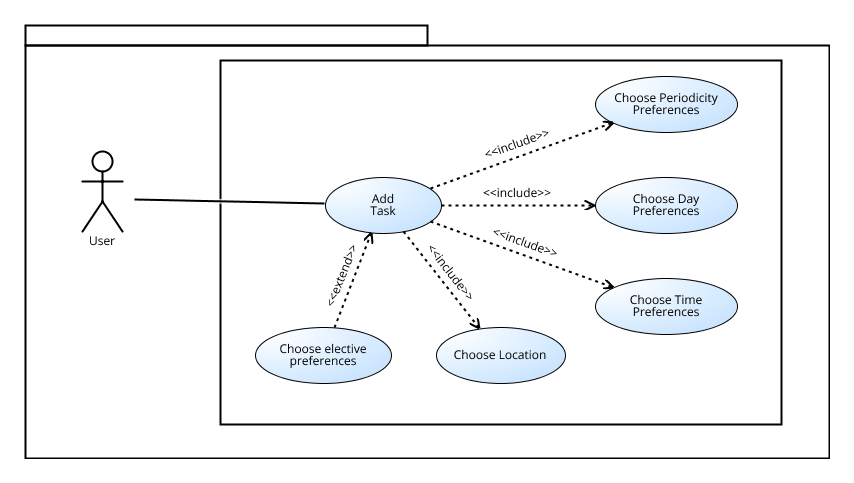
\includegraphics[scale=0.5]{Pictures/UseCaseDiagram/Adding_a_new_task.png}
\caption{UML Use Case Diagram for the addition of a new task }
\end{figure}

\begin{figure}[H]
\centering
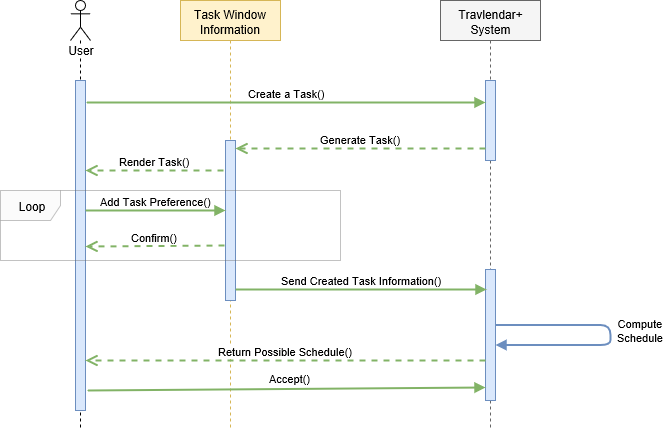
\includegraphics[scale=0.5]{Pictures/SequenceDiagram/adding_a_task.png}
\caption{UML Sequence Diagram for the addition of a new task, \emph{without overlapping}}
\end{figure}

\begin{figure}[H]
\centering
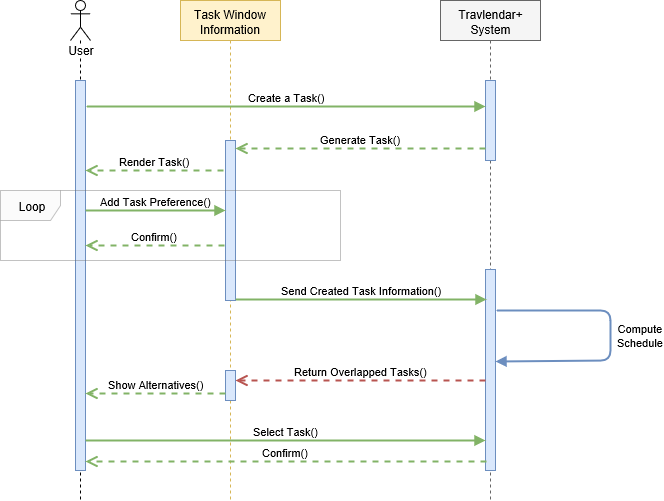
\includegraphics[scale=0.5]{Pictures/SequenceDiagram/adding_a_task_with_overlapping.png}
\caption{UML Sequence Diagram for the addition of a new task, \emph{with overlapping}}
\end{figure}